\documentclass{../vespers-booklet}
\usepackage{multicol}

\begin{document}

% TODO: Update the title for the specific feast
\chapter*{Second Vespers of the Ascension of Our Lord}

\begin{center}
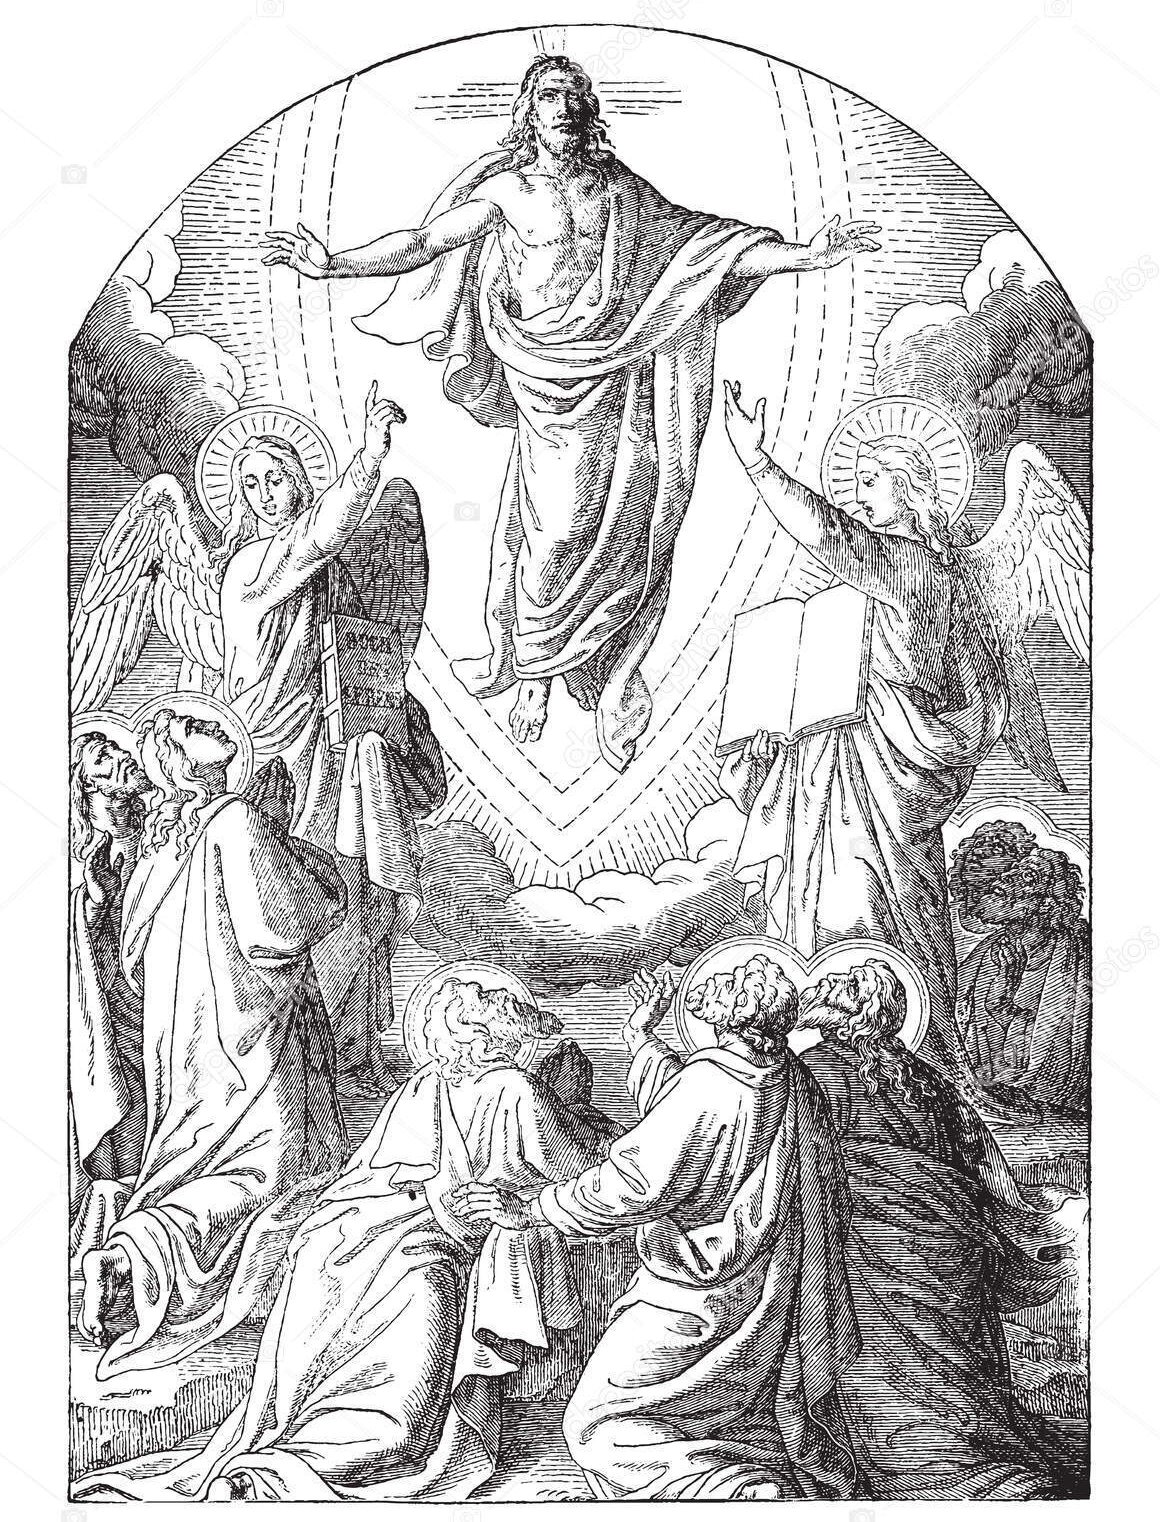
\includegraphics[width=0.7\linewidth]{ascension_line_art}
\end{center}

\vfill\newpage

%\section*{Beginning of the Office}

\begin{rubricbox}

{\color{red}When the Officiant kneels, all \textbf{kneel} and pray silently.
Then, when the Officiant stands, all \textbf{stand} and say silently one \textit{Pater noster} (Our Father) and \textit{Ave Maria} (Hail Mary).
Then all make the sign of the cross with the Officiant as he intones:}

\end{rubricbox}

% TODO: Make sure that the tone of the deus adjutorium matches the season primarily and the solemnity of the feast secondarily
 \gresetinitiallines{1}
\gregorioscore{../common/deus-in-adjutorium-solemn}

\textit{
O God, come to my assistance.
{\color{red}\Vbar.}~O Lord, make haste to help me.
Glory be to the Father, and to the Son, and to the Holy Spirit,
as it was in the beginning, is now, and ever shall be, world without end. Amen.
Praise to Thee, O Lord, King of endless glory.}

%TODO: Add that the correct psalms, and verify that their tones, and their associated pointed text are correct

\section*{Psalm 109}

\textit{\textnormal{Ant. 1.} Men of Galilee, why do you stand looking up to heaven? This Jesus who has been take up from you into heaven, will come in the same way as you have seen Him going up to heaven, alleluia.
 \textnormal{Ps.} The Lord said to my Lord...}
 
 \begin{rubricbox}

{\color{red}All remain standing throughout the first antiphon.
After the psalm is intoned by the Cantor, all \textbf{sit} at the asterisk.}

\end{rubricbox}

\gresetinitiallines{1}
\gregorioscore{ps109-antiphon}

\gresetinitiallines{0}
\gregorioscore{ps109-intonation}

 \begin{latinenglishsection}

\latinenglish{

	2. Donec ponam ini\textbf{mí}cos \textbf{tu}os,~* scabéllum \textbf{pe}dum tu\textbf{ó}rum.

3. Virgam virtútis tuæ emíttet Dómi\textbf{nus} ex \textbf{Si}on:~* domináre in médio inimi\textbf{có}rum tu\textbf{ó}rum.

4. Tecum princípium in die virtútis tuæ in splendóri\textbf{bus} sanc\textbf{tó}rum:~* ex útero ante lucíferum \textbf{gé}nu\textbf{i} te.

5. Jurávit Dóminus, et non poeni\textbf{té}bit \textbf{e}um:~* Tu es sacérdos in ætérnum secúndum órdi\textbf{nem} Mel\textbf{chí}sedech.

6. Dóminus a \textbf{dex}tris \textbf{tu}is,~* confrégit in die iræ \textbf{su}æ \textbf{re}ges.

7. Judicábit in natiónibus, im\textbf{plé}bit ru\textbf{í}nas:~* conquassábit cápita in \textbf{ter}ra mul\textbf{tó}rum.

8. De torrénte in \textbf{vi}a \textbf{bi}bet:~* {\color{red}\textit{(stand)}} proptérea exal\textbf{tá}bit \textbf{ca}put.

{\color{red}\textit{(bow)}} Glória \textbf{Pa}tri, et \textbf{Fí}lio,~* et Spi\textbf{rí}tui \textbf{Sanc}to.

{\color{red}\textit{(rise)}} Sicut erat in princípio, et \textbf{nunc}, et \textbf{sem}per,~* et in s\'{\ae}cula sæcu\textbf{ló}rum. \textbf{A}men. %%

}{
	% 1. The Lord said to my Lord: Sit thou at my right hand:

2. Until I make thy enemies thy footstool.
 
3. The Lord will send forth the sceptre of thy power out of Sion: rule thou in the midst of thy enemies.
 
4. With thee is the principality in the day of thy strength: in the brightness of the saints:
 from the womb before the day star I begot thee.
 
5. The Lord hath sworn, and he will not repent: Thou art a priest for ever according to the order of Melchisedech.
 
6. The Lord at thy right hand hath broken kings in the day of his wrath.

7. He shall judge among nations, he shall fill ruins: he shall crush the heads in the land of the many.

8. He shall drink of the torrent in the way: therefore shall he lift up the head. 

Glory be. %%
}

\end{latinenglishsection}

\begin{rubricbox}

{\color{red}The antiphon is repeated: Viri Galilei\textit{\dots}} %%

\end{rubricbox}

\section*{Psalm 110}

\textit{\textnormal{Ant. 2.} While they were beholding Him going up to heaven, they said, alleluia.
 \textnormal{Ps.} I praise Thee, O Lord, with all my heart...}

\gresetinitiallines{1}
\gregorioscore{ps110-antiphon}

\gresetinitiallines{0}
\gregorioscore{ps110-intonation}

 \begin{latinenglishsection}

\latinenglish{

	2. Magna ópera \textbf{Dó}mini:~* exquisíta in omnes volun\textit{tá}\textit{tes} \textbf{e}jus.

3. Conféssio et magnificéntia opus \textbf{e}jus:~* et justítia ejus manet in sǽ\textit{cu}\textit{lum} \textbf{sǽ}culi.

4. Memóriam fecit mirabílium suórum,~{\color{red}\GreDagger} miséricors et miserátor \textbf{Dó}minus:~* escam dedit ti\textit{mén}\textit{ti}\textbf{bus} se.

5. Memor erit in sǽculum testaménti \textbf{su}i:~* virtútem óperum suórum annuntiábit pó\textit{pu}\textit{lo} \textbf{su}o:

6. Ut det illis hereditátem \textbf{gén}tium:~* ópera mánuum ejus véritas, \textit{et} \textit{ju}\textbf{dí}cium.

7. Fidélia ómnia mandáta ejus:~{\color{red}\GreDagger} confirmáta in sǽculum \textbf{sǽ}culi,~* facta in veritáte et \textit{æ}\textit{qui}\textbf{tá}te.

8. Redemptiónem misit pópulo \textbf{su}o:~* mandávit in ætérnum testa\textit{mén}\textit{tum} \textbf{su}um.

9. Sanctum, et terríbile nomen \textbf{e}jus:~* inítium sapiéntiæ \textit{ti}\textit{mor} \textbf{Dó}mini.

10. Intelléctus bonus ómnibus faciéntibus \textbf{e}um:~* laudátio ejus manet in sǽ\textit{cu}\textit{lum} \textbf{sǽ}culi.

{\color{red}\textit{(bow)}} Glória Patri, et \textbf{Fí}lio,~* et Spirí\textit{tu}\textit{i} \textbf{Sanc}to.

{\color{red}\textit{(rise)}} Sicut erat in princípio, et nunc, et \textbf{sem}per,~* et in s\'{\ae}cula sæcu\textit{ló}\textit{rum}. \textbf{A}men.
 %%

}{
	 1. I will praise thee, O Lord, with my whole heart; in the council of the just: and in the congregation.
 
 2. Great are the works of the Lord: sought out according to all his wills.
 
 3. His work is praise and magnificence: and his justice continueth for ever and ever.
 
 4.  He hath made a remembrance of his wonderful works, being a merciful and gracious Lord: he hath given food to them that fear him. 	
 
 5. He will be mindful for ever of his covenant: he will shew forth to his people the power of his works.
 
 6. That he may give them the inheritance of the Gentiles: the works of his hands are truth and judgment.
 
 7. All his commandments are faithful: confirmed for ever and ever, made in truth and equity.
 
 8. He hath sent redemption to his people: he hath commanded his covenant for ever.
 
 9. Holy and terrible is his name: the fear of the Lord is the beginning of wisdom.
 
 10. A good understanding to all that do it: his praise continueth for ever and ever.  %%
}

\end{latinenglishsection}

\begin{rubricbox}

{\color{red}The antiphon is repeated: Cumque intueréntur\textit{\dots}} %%

\end{rubricbox}

\section*{Psalm 111}

\textit{\textnormal{Ant. 3.} Lifting up his hands, He blessed them and was carried up to heaen, alleluia.
 \textnormal{Ps.} Blessed is the man that feareth the Lord...}

\gresetinitiallines{1}
\gregorioscore{ps111-antiphon}

\gresetinitiallines{0}
\gregorioscore{ps111-intonation}

 \begin{latinenglishsection}

\latinenglish{

	2. Potens in terra erit \textit{se}\textit{men} \textbf{e}jus:~* generátio rectórum \textit{be}\textit{ne}\textit{di}\textbf{cé}tur.

3. Glória, et divítiæ in \textit{do}\textit{mo} \textbf{e}jus:~* et justítia ejus manet in \textit{sǽ}\textit{cu}\textit{lum} \textbf{sǽ}culi.

4. Exórtum est in ténebris \textit{lu}\textit{men} \textbf{rec}tis:~* miséricors, et mise\textit{rá}\textit{tor}, \textit{et} \textbf{jus}tus.

5. Jucúndus homo qui miserétur et cómmodat,~{\color{red}\GreDagger} dispónet sermónes suos \textit{in} \textit{ju}\textbf{dí}cio:~* quia in ætérnum \textit{non} \textit{com}\textit{mo}\textbf{vé}bitur.

6. In memória ætérna \textit{e}\textit{rit} \textbf{jus}tus:~* ab auditióne ma\textit{la} \textit{non} \textit{ti}\textbf{mé}bit.

7. Parátum cor ejus speráre in Dómino,~{\color{red}\GreDagger} confirmátum \textit{est} \textit{cor} \textbf{e}jus:~* non commovébitur donec despíciat in\textit{i}\textit{mí}\textit{cos} \textbf{su}os.

8. Dispérsit, dedit paupéribus:~{\color{red}\GreDagger} justítia ejus manet in sǽ\textit{cu}\textit{lum} \textbf{sǽ}culi,~* cornu ejus exaltá\textit{bi}\textit{tur} \textit{in} \textbf{gló}ria.

9. Peccátor vidébit, et irascétur,~{\color{red}\GreDagger} déntibus suis fremet \textit{et} \textit{ta}\textbf{bé}scet:~* desidérium pecca\textit{tó}\textit{rum} \textit{per}\textbf{í}bit.

{\color{red}\textit{(bow)}} Glória Pa\textit{tri}, \textit{et} \textbf{Fí}lio,~* et Spi\textit{rí}\textit{tu}\textit{i} \textbf{Sanc}to.

{\color{red}\textit{(rise)}} Sicut erat in princípio, et \textit{nunc}, \textit{et} \textbf{sem}per,~* et in s\'{\ae}cula sæ\textit{cu}\textit{ló}\textit{rum}. \textbf{A}men.
 %%

}{
	1. Blessed is the man that feareth the Lord: he shall delight exceedingly in his commandments.

2. His seed shall be mighty upon earth: the generation of the righteous shall be blessed.

3. Glory and wealth shall be in his house: and his justice remaineth for ever and ever.

4. To the righteous a light is risen up in darkness: he is merciful, and compassionate and just.

5. Acceptable is the man that sheweth mercy and lendeth: he shall order his words with judgment:
because he shall not be moved for ever.

6. The just shall be in everlasting remembrance: he shall not fear the evil hearing.

7. His heart is ready to hope in the Lord: his heart is strengthened, he shall not be moved until he look over his enemies.

8. He hath distributed, he hath given to the poor: his justice remaineth for ever and ever: his horn shall be exalted in glory.

9. The wicked shall see, and shall be angry, he shall gnash with his teeth and pine away: the desire of the wicked shall perish.  %%
}

\end{latinenglishsection}

\begin{rubricbox}

{\color{red}The antiphon is repeated: Elevátis mánibus\textit{\dots}} %%

\end{rubricbox}

\vfill\pagebreak

\section*{Psalm 112}

\textit{\textnormal{Ant. 4.} While they were looking on, He was raised up and a cloud received Him into heaven, alleluia.
 \textnormal{Ps.} Praise the Lord, ye children...}

\gresetinitiallines{1}
\gregorioscore{ps112-antiphon}

\gresetinitiallines{0}
\gregorioscore{ps112-intonation}

 \begin{latinenglishsection}

\latinenglish{

	2. Sit nomen Dómini bene\textbf{díc}tum,~* ex hoc nunc, et us\textit{que} \textit{in} \textbf{sǽ}culum.

3. A solis ortu usque ad oc\textbf{cá}sum,~* laudábile \textit{no}\textit{men} \textbf{Dó}mini.

4. Excélsus super omnes gentes \textbf{Dó}minus,~* et super cælos gló\textit{ri}\textit{a} \textbf{e}jus.

5. Quis sicut Dóminus, Deus noster, qui in altis \textbf{há}bitat,~* et humília réspicit in cælo \textit{et} \textit{in} \textbf{ter}ra?

6. Súscitans a terra \textbf{ín}opem,~* et de stércore é\textit{ri}\textit{gens} \textbf{páu}perem:

7. Ut cóllocet eum cum prin\textbf{cí}pibus,~* cum princípibus pó\textit{pu}\textit{li} \textbf{su}i.

8. Qui habitáre facit stérilem in \textbf{do}mo,~* matrem filió\textit{rum} \textit{læ}\textbf{tán}tem.

{\color{red}\textit{(bow)}} Glória Patri, et \textbf{Fí}lio,~* et Spirí\textit{tu}\textit{i} \textbf{Sanc}to.

{\color{red}\textit{(rise)}} Sicut erat in princípio, et nunc, et \textbf{sem}per,~* et in s\'{\ae}cula sæcu\textit{ló}\textit{rum}. \textbf{A}men.
 %%

}{
	%1. Praise the Lord, ye children: praise ye the name of the Lord.
 	
2. Blessed be the name of the Lord, from henceforth now and for ever.
 	
3. From the rising of the sun unto the going down of the same, the name of the Lord is worthy of praise.
 	
4. The Lord is high above all nations; and his glory above the heavens.
 	
5.Who is as the Lord our God, who dwelleth on high, and looketh down on the low things in heaven and in earth?
 	
6. Raising up the needy from the earth, and lifting up the poor out of the dunghill:
 	
7. That he may place him with princes, with the princes of his people.
 	
8. Who maketh a barren woman to dwell in a house, the joyful mother of children. 

Glory be. %%
}

\end{latinenglishsection}

\begin{rubricbox}

{\color{red}The antiphon is repeated: Vidéntibus illis\textit{\dots}} %%

\end{rubricbox}


%TODO: Verify that the little chapter is fitting for the feast

\section*{Chapter (Acts 1, 1-2)}

\textit{\color{red}The Officiant leads the Little Chapter:}

\begin{latinenglishsection}

\latinenglish{
	Primum quiden sermónem feci dei ómnibus, o Theóphile, qu\ae c\oe pit Iesus fácere et docére {\color{red}\GreDagger} usque in diem, qua pr\ae cipiens Apóstolis per Spiritum Sanctum, quos elégit, {\color{red}*} assumptus est.
}{
	In the former book, O Theophilus, I spoke of all that Jesus did and taught from the beginning, until the day on which He was taken up, after He had given commandments through the Holy Spirit to the Apostles, whom He had chosen.
}

\end{latinenglishsection}

\subsection*{Short Responsory}

\gresetinitiallines{0}
\gregorioscore{short_responsory}
\textit{{\color{red}\Vbar.} When Christ ascended up on high. * Alleluia, alleluia.
{\color{red}\Rbar.} When Christ ascended up on high. * Alleluia, alleluia.
{\color{red}\Vbar.} He led captivity captive. {\color{red}\Rbar.} Alleluia, alleluia.
{\color{red}\Vbar.} Glory be to the Father, and to the Son, * and to the Holy Ghost.
{\color{red}\Rbar.} When Christ ascended up on high. * Alleluia, alleluia.}

% TODO: Verify that the hymn is correct for the feast (including the responsory after the hymn)

\section*{Hymn}

\textit{\color{red}The Cantor leads the hymn:}

\gresetinitiallines{1}
\gregorioscore{../hymns/iesu_nostra_redemptio}

{\itshape

   1.  Jesus, Redemption all divine,
   Whom her we love, for Whom we pine,
   God, working out creation's plan
   And in the latter time made Man;
    
   2.  What love of Thine was that, which led
   To take our woes upon Thy head
   And pangs and cruel death to bear
   To ransomus from death's despair.
    
    3. To Thee hell's gate gave ready way,
    Demanding there his captive prey;
    And now in pomp and victor's pride
    Thou sittest at They Father's side.
    
   4.  Let very mercy force Thee still
   To spare us, conquering all our ill;
   And, granting what we ask, on high
   With Thine own face to satisfy.
    
    5. Be Thou our joy and Thou our guard,
    Who art to be our great reward;
    Our glory and our boast in Thee
    Forever and forever be.
    Amen.
}

\textit{\color{red}The Cantor says the following before all reply afterwards:}

\gresetinitiallines{0}
\gabcsnippet{
(c3) <c><sp>V/</sp>.</c> A(h)scen(h)dit(h) De(h)us(h) in(h) ju(h)bi(h)la(h)ti(h)o(hi)ne(h_'),(,) al(h)le(fe)lu(fh_)i(hi)a(H'Ghih.ghG'FEfgge.). (::)
}

\gresetinitiallines{0}
\gabcsnippet{
(c3) <c><sp>R/</sp>.</c> Et(h) Do(h)mi(h)nus(h) in(h) vo(h)ce(h) tu(hi)bæ(h_'),(,)  al(h)le(fe)lu(fh_)i(hi)a(H'Ghih.ghG'FEfgge.). (::)
}

\textit{{\color{red}\Vbar.}~God ascends amid shouts of triumph, alleluia.
{\color{red}\Rbar.}~And the Lord with the sound of trumpets, alleluia.}

%TODO: Verify that the magnificat antiphon is correct and match the mangificat intonation and pointed text with the tone

\section*{Magnificat}

\textit{\textnormal{Ant Magn.}  O King of glory, Lord of hosts, * Who hast this day exalted thine Own Self, with great triumph, above all the heavens, leave us not orphans but send unto us the Promise of the Father, even the Spirit of truth, alleluia.
\textnormal{Cant.} My soul doth magnify the Lord: and my spirit hath rejoiced in God my Saviour...}

\begin{rubricbox}

{\color{red}The Cantor leads by intoning the antiphon and the first verse.}

\end{rubricbox}

\gresetinitiallines{1}
\gregorioscore{magnificat-antiphon-only}

\begin{rubricbox}

{\color{red}All \textbf{stand} and make the sign of the cross with the Cantor.}

\end{rubricbox}

\gresetinitiallines{0}
\gregorioscore{magnificat-intonation}

 \begin{latinenglishsection}

\latinenglish{	
3. Quia respéxit humilitátem ancíllæ \textbf{su}æ:~* 
ecce enim ex hoc beátam me dicent omnes genera\textit{ti}\textbf{ó}nes.

4. Quia fecit mihi magna qui \textbf{pot}ens est:~* 
et sanctum no\textit{men} \textbf{e}jus.

5. Et misericórdia ejus a progénie in pro\textbf{gé}nies~* 
timénti\textit{bus} \textbf{e}um.

6. Fecit poténtiam in bráchio \textbf{su}o:~* 
dispérsit supérbos mente cor\textit{dis} \textbf{su}i.

7. Depósuit poténtes de \textbf{se}de,~* 
et exaltá\textit{vit} \textbf{hú}\textbf{mi}les.

8. Esuriéntes implévit \textbf{bo}nis:~* 
et dívites dimísit \textit{in}\textbf{á}nes.

9. Suscépit Israël púerum \textbf{su}um,~* 
recordátus misericórdi\textit{æ} \textbf{su}æ.

10. Sicut locútus est ad patres \textbf{nos}tros,~* 
Abraham et sémini ejus \textit{in} \textbf{s\'{\ae}}\textbf{cu}la.
}{	
	1. My soul doth magnify the Lord.

2. And my spirit hath rejoiced in God my Saviour.

3. Because he hath regarded the humility of his handmaid; for behold from henceforth all generations shall call me blessed.

4. Because he that is mighty, hath done great things to me; and holy is his name.

5. And his mercy is from generation unto generations, to them that fear him.

6. He hath shewed might in his arm: he hath scattered the proud in the conceit of their heart.

7. He hath put down the mighty from their seat, and hath exalted the humble.

8. He hath filled the hungry with good things; and the rich he hath sent empty away.

9. He hath received Israel his servant, being mindful of his mercy: 

10. As he spoke to our fathers, to Abraham and to his seed for ever. 
}

\end{latinenglishsection}

\textit{\color{red}(bow)} Glória Patri, et \textbf{Fí}lio,~* 
et Spirítu\textit{i} \textbf{Sanc}to.

\textit{\color{red}(rise)} Sicut erat in princípio, et nunc, et \textbf{sem}per,~*
et in s\'{\ae}cula sæculó\textit{rum}. \textbf{A}men.

\begin{rubricbox}

{\color{red}All \textbf{remain standing} and repeat the antiphon: O Rex gloriae\textit{\dots}, %%
then \textbf{stand} for the prayer.}

\end{rubricbox}

\gresetinitiallines{1}
\gregorioscore{../common/kyrie_eleison_simplex}

%TODO: Add commemorations for the date

%\textit{\color{red}For commemorations, the Cantor intones the antiphon and says the responsorial prayer afterwards. The Officiant prays the associated collect.}
%
%\gresetinitiallines{1}
%\gregorioscore{commemoration}
%

%\vfill\pagebreak

\textit{\color{red}The Officiant leads the following, saying the Pater Noster aloud:}

\begin{latinenglishsection}

\latinenglish{
	Pater noster, qui es in cælis, sanctificétur nomen tuum: advéniat regnum tuum: fiat volúntas tua, sicut in cælo et in terra. Panem nostrum cotidiánum da nobis hódie: et dimítte nobis débita nostra, sicut et nos dimíttimus debitóribus nostris:\\
	{\color{red}\Vbar.} Et ne nos indúcas in tentatiónem:
	
	{\color{red}\Rbar.} Sed líbera nos a malo.
}{
	Our Father, who art in heaven, Hallowed be thy name. Thy kingdom come. Thy will be done on earth as it is in heaven. Give us this day our daily bread. And forgive us our trespasses, as we forgive those who trespass against us.\\
	{\color{red}\Vbar.} And lead us not into temptation: 
	
	{\color{red}\Rbar.} But deliver us from evil.
}

\end{latinenglishsection}

\vfill\pagebreak

%TODO: Verify (with the antiphonary) that the collect is proper for the season. If it is not in antiphonary, use the missal for the feast.

\section*{Collect}

\textit{\color{red}The Officiant leads the collect:}

\begin{latinenglishsection}

\latinenglish{
	{\color{red}\Vbar.}~Dómine exáudi oratiónem meam.\\
	{\color{red}\Rbar.}~Et clamor meus ad te véniat.
	
	Orémus.
	Concéde, qu\'{\ae}sumus, omnípotens Deus: ut, qui hodiérna die Unigénitum tuum, Redemptórem nostrum, ad cælos ascendísse crédimus; ipsi quoque mente in cæléstibus habitémus.\\
	Per eúndem Dóminum nostrum Iesum Christum Fílium tuum, qui tecum vivit et regnat in unitáte Spíritus Sancti, Deus, per ómnia s\'{\ae}cula sæculórum.\\
	{\color{red}\Rbar.}~Amen.
}{
	{\color{red}\Vbar.} O Lord, hear my prayer.
	{\color{red}\Rbar.}~And let my cry come unto Thee.
	
	Let us pray.
	Grant, we beseech thee, Almighty God, that just as we do believe thine Only-Begotten Son, our Saviour, to have this day ascended into the heavens, so we may also in heart and mind thither ascend, and with Him continually dwell.\\
	Through the same Jesus Christ, thy Son, Our Lord, Who liveth and reigneth with thee in the unity of the Holy Ghost, God, world without end. \\
	{\color{red}\Rbar.}~Amen.
}
\end{latinenglishsection}

%TODO: Add the Marian Anthem for the season and verify that the oration afterwards is correct

%\section*{Marian Anthem}
%
%\textit{\color{red}The Cantor leads the Marian anthem and responses afterwards; the Officiant leads the ending collect:}
%
%\gresetinitiallines{1}
%\gregorioscore{../marian-anthems/regina-caeli-solemn}
%
%{\itshape
%	Queen of heaven, rejoice, alleluia; 
%	for He whom thou was chosen to bear, alleluia; 
%	has risen as He said, alleluia; 
%	pray for us to God, alleluia.
%}
%
%\begin{latinenglishsection}
%
%\latinenglish{
%	{\color{red}\Vbar.} Gaude et laetare, Virgo Maria, alleluia. \\
%	{\color{red}\Rbar.} Quia surrexit Dominus vere, alleluia.
%	
%	Orémus.
%	 Deus, qui per resurrectionem Filii tui, Domini nostri Iesu Christi, mundum laetificare dignatus es: praesta, quaesumus; ut per eius Genetricem Virginem Mariam, perpetuae capiamus gaudia vitae. 
%	 Per eundem Christum Dominum nostrum. Amen.
%	{\color{red}\Rbar.}~Amen.
%}{
%	{\color{red}\Vbar.}Rejoice and be glad, O Virgin Mary, alleluia.
%	{\color{red}\Rbar.}~For the Lord has truly risen, alleluia.
%	
%	Let us pray. 
%	O God, who gave joy to the world through the resurrection of Thy Son, our Lord Jesus Christ, grant we beseech Thee, that through the intercession of the Virgin Mary, His Mother, we may obtain the joys of everlasting life. 
%	Through the same Christ our Lord. Amen.
%	{\color{red}\Rbar.}~Amen.
%}
%\end{latinenglishsection}

\textit{\color{red}The Officiant leads the following:}

\begin{latinenglishsection}

\latinenglish{
	{\color{red}\Vbar.} Dómine, exáudi oratiónem meam.
	{\color{red}\Rbar.} Et clamor meus ad te véniat.
}{
	{\color{red}\Vbar.} O Lord, hear my prayer.
	{\color{red}\Rbar.} And let my cry come unto thee.
}

\end{latinenglishsection}

\textit{\color{red}The Cantor leads the Benedicamus:}

\gresetinitiallines{1}
\gregorioscore{../common/benedicamus-2v-solem}

\begin{latinenglishsection}	

\latinenglish{
	{\color{red}\Vbar.} Fidélium ánimæ per misericórdiam Dei requiéscant in pace.\\
	{\color{red}\Rbar.} Amen.

	{\color{red}\Vbar.} Divínum auxílium {\color{red}\maltese} máneat semper nobíscum.\\
	{\color{red}\Rbar.} Amen.
}{
	{\color{red}\Vbar.} May the souls of the faithful, through the mercy of God, rest in peace.
	{\color{red}\Rbar.} Amen.
	
	{\color{red}\Vbar.} May the divine assistance remain always with us.
	{\color{red}\Rbar.}~Amen.
}
\end{latinenglishsection}

\begin{rubricbox}

{\color{red} After the Office, all \textbf{kneel} and pray in silence for a time.}

\end{rubricbox}

\end{document}